\documentclass[../../main.tex]{subfiles}
\graphicspath{{\subfix{../images/}}} % 指定图片目录,后续可以直接使用图片文件名。
\begin{document}
\section{Homework 5}
\subsection{Partition Function}
\textbf{Show that the partition function of an Ising lattice can be written as
  \begin{align*}
    Q_{N}(B,T) = \sum_{N_{+},N_{+-}} g_{N}(N_{+},N_{+-}) \text{exp}\{-\beta H_{N}(N_{+},N_{+-})\},
  \end{align*}
  where
  \begin{align}
    H_{N}(N_{+},N_{+-}) = -J \left(\frac{1}{2}qN - 2N_{+-}\right) - \mu B(2N_{+}-N),\label{eq:1}
  \end{align}
  while other symbols have their usual meanings; compare these results to equations 
  \begin{align}
    H_{N}(N_{+},N_{++}) &= -J(N_{++}+N_{--}-N_{+-})-\mu B(N_{+}-N_{-})\\
    &= -J\left(\frac{1}{2}qN - 2qN_{+} + 4N_{++}\right) - \mu B(2N_{+}-N)\label{eq:2}
  \end{align} and 
  \begin{align*}
    Q_{N}(B,T) = \sum_{N_{+},N_{++}}g_{N}(N_{+},N_{++})\text{exp }\{-\beta H_{N}(N_{+},N_{++})\}.
  \end{align*}}

  The Hamiltonian of the Ising model is given by
  \begin{align*}
    H = -J\sum_{\langle i,j\rangle}\sigma_{i}\sigma_{j}- \mu B\sum_{i}\sigma_{i},\quad \sigma_{i} = \pm 1 \quad\forall i.
  \end{align*}
  The total number of neighbor pairs is 
  \begin{align*}
    N_{++} + N_{--} + N_{+-} = \frac{1}{2}qN
  \end{align*}
  So the interaction energy component of the Hamiltonian becomes 
  \begin{align*}
    -J\sum_{\langle i,j\rangle}\sigma_{i}\sigma_{j} = -J(N_{++}+N_{--}-N_{+-}),
  \end{align*}
  where $\sigma_{i}\sigma_{j} = +1$ for $N_{++}$ and $N_{--}$, and $\sigma_{i}\sigma_{j} = -1$ for $N_{+-}$. 

  The magnetic energy component is 
\begin{align*}
  -\mu B\sum_{i}\sigma_{i} = -\mu B(N_{+}-N_{-}) = -\mu B(2N_{+}-N),\quad N_{-} = N - N_{+}. 
\end{align*}

Combining these two components gives the total Hamiltonian
\begin{align*}
  H_{N} = -J(N_{++}+N_{--}-N_{+-}) - \mu B(2N_{+}-N)
\end{align*}
Using the relation $\begin{aligned}
  N_{++} + N_{--} = \frac{1}{2}qN - N_{+-}
\end{aligned}$, we can rewrite the Hamiltonian as
\begin{align*}
  \boxed{H_{N} = -J\left(\frac{1}{2}qN - 2N_{+-}\right) - \mu B(2N_{+}-N)},
\end{align*}
So the partition function can be expressed as
\begin{align*}
  Q_{N}(B,T) &= \sum_{N_{+},N_{+-}} g_{N}(N_{+},N_{+-}) \text{exp}\{-\beta H_{N}(N_{+},N_{+-})\}\\ 
  &= \sum_{N_{+},N_{+-}} g_{N}(N_{+},N_{+-}) \text{exp}\left\{-\beta \left[-J\left(\frac{1}{2}qN - 2N_{+-}\right) - \mu B(2N_{+}-N)\right]\right\}
\end{align*}
which matches the provided expression.

To prove that \eqref{eq:1} and \eqref{eq:2} are equivalent, we can use the relation between $N_{+-}$ and $N_{++}$:
\begin{align*}
  qN_{+} = 2N_{++} + N_{+-} \Rightarrow N_{+-} = qN_{+} - 2N_{++}
\end{align*}
Substituting this into \eqref{eq:1} gives:
\begin{align*}
  H_{N}(N_{+},N_{+-}) &= -J\left[\frac{1}{2}qN - 2(qN_{+} - 2N_{++})\right] - \mu B(2N_{+}-N)\\
  &= \boxed{-J\left(\frac{1}{2}qN - 2qN_{+} + 4N_{++}\right) - \mu B(2N_{+}-N)}
\end{align*}

\subsection{Equation of State}
\textbf{Show that the curve in \ref{fig:12.7} hits the horizontal and vertical axes at right angle according to the equation of state 
  \begin{align*}
    \bar{L}_{0} = \tanh{\left(\frac{qJ\bar{L}_{0}}{kT}\right)}.
  \end{align*}}
  
  	\begin{figure} 
		\centering
		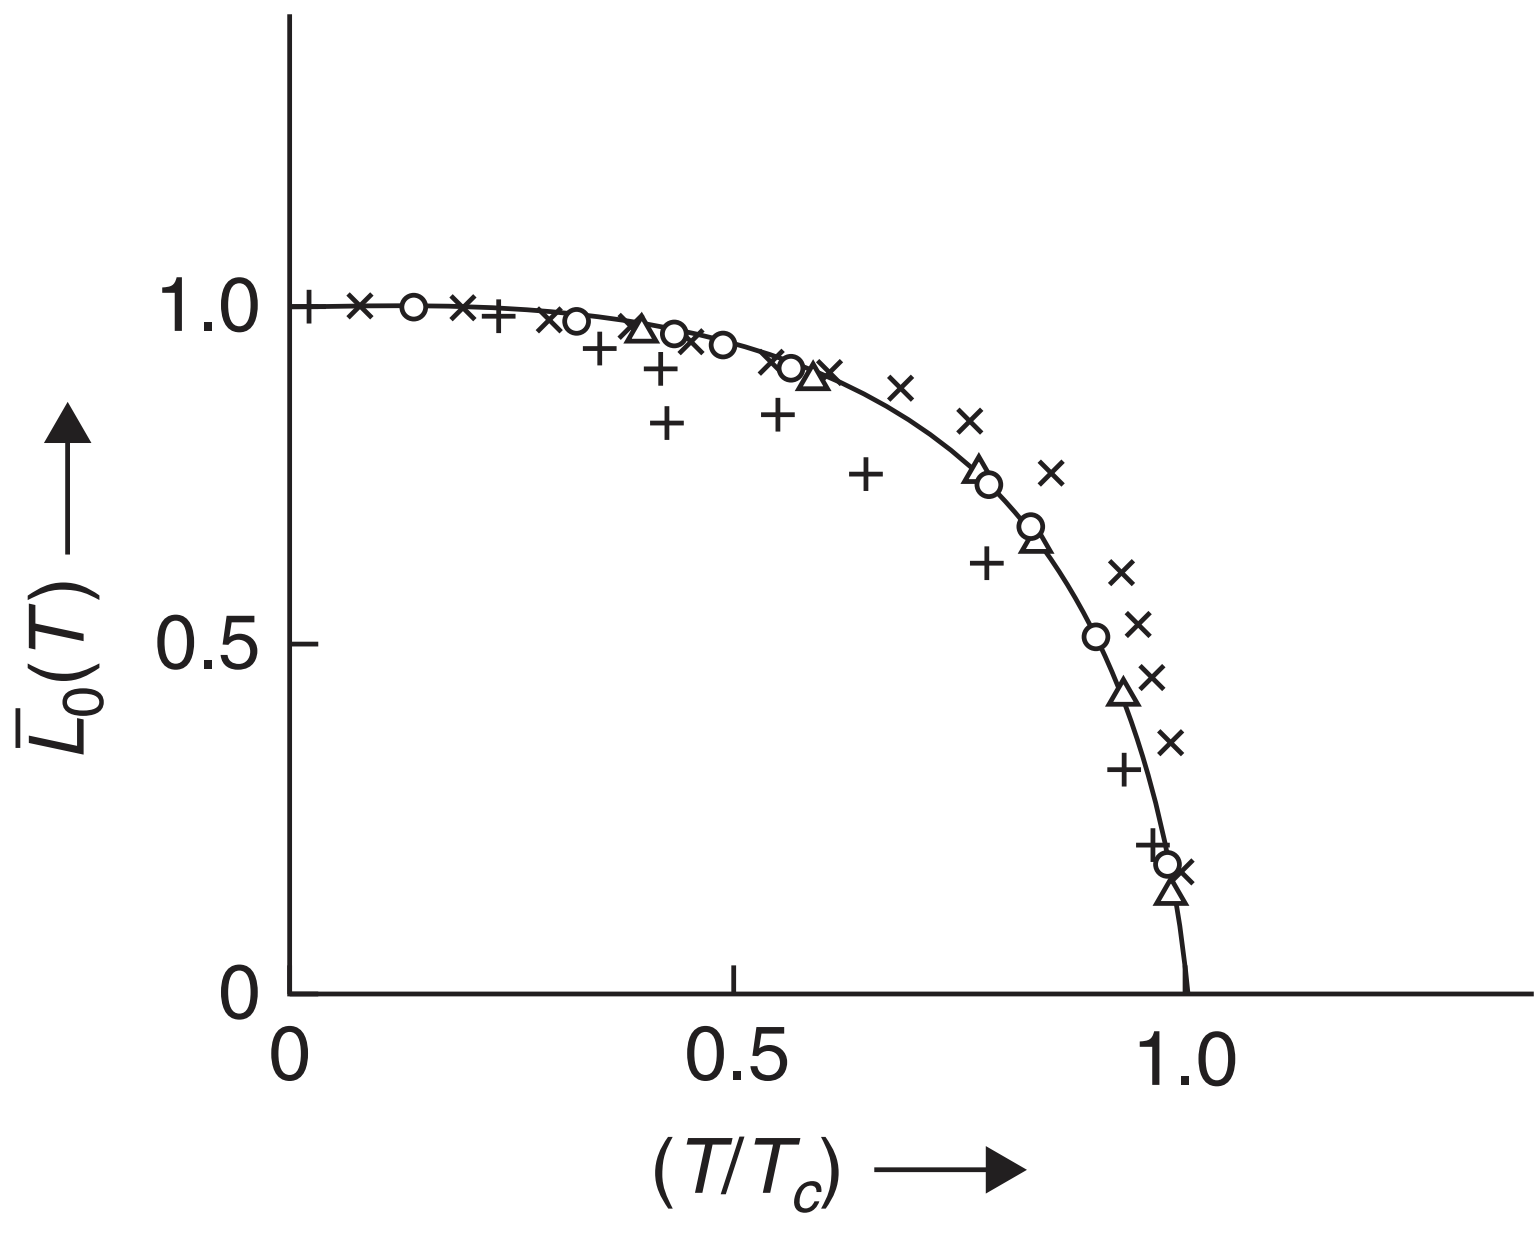
\includegraphics[width=0.33\textwidth,height=0.3\textwidth]{fig/fig.png}
    \caption{The spontaneous magnetization of a Weiss ferromagnet as a function of temperature. The experimental points (after Becker) are for iron (x), nickel (o), cobalt ($\Delta$), and magnetite (+).} \label{fig:12.7}
	\end{figure}

  To show that the curve given by the equation of state $\begin{aligned}
    \bar{L}_{0} = \tanh{\left(\frac{qJ\bar{L}_{0}}{kT}\right)} 
  \end{aligned}$ hits the horizontal and vertical axes at right angles, we need to analyze the slope of the curve at the boundaries($T = 0$ and $\begin{aligned}
      T = T_{c} = \frac{qJ}{k}
    \end{aligned}$).

    Differentiate both sides of the equation with respect to $T$, with chain rule:
    \begin{align*}
      \frac{\mathrm{d}\bar{L}_{0}}{\mathrm{d}T} &= \sech^{2}\left(\frac{qJ\bar{L}_{0}}{kT}\right)\left(\frac{qJ}{kT}\frac{\mathrm{d}\bar{L}_{0}}{\mathrm{d}T} - \frac{qJ\bar{L}_{0}}{kT^{2}}\right)\\
      \left[ 1 - \sech^{2}\left(\frac{qJ\bar{L}_{0}}{kT}\right)\frac{qJ}{kT}\right]\frac{\mathrm{d}\bar{L}_{0}}{\mathrm{d}T} &= -\sech^{2}\left(\frac{qJ\bar{L}_{0}}{kT}\right)\frac{qJ\bar{L}_{0}}{kT^{2}}\\
      \frac{\mathrm{d}\bar{L}_{0}}{\mathrm{d}T} &= \frac{\sech^{2}\left(\frac{qJ\bar{L}_{0}}{kT}\right)\frac{qJ\bar{L}_{0}}{kT^{2}}}{\sech^{2}\left(\frac{qJ\bar{L}_{0}}{kT}\right)\frac{qJ}{kT}-1}
    \end{align*}

  \begin{enumerate}
    \item At $T = 0$. Define $\begin{aligned}
      x = \frac{qJ\bar{L}_{0}}{kT}
    \end{aligned}$, we have: 
    \begin{align*}
      \lim_{T\rightarrow 0}\tanh{\left(\frac{qJ\bar{L}_{0}}{kT}\right)} &= \lim_{x\rightarrow \infty}\tanh{x} = 1, \quad\forall \bar{L}_{0}\neq 0\\
      &\Rightarrow  \lim_{T\rightarrow 0}\bar{L}_{0} = 1 \\
      \lim_{T\rightarrow 0}\sech^{2}\left(\frac{qJ\bar{L}_{0}}{kT}\right) &= \lim_{x\rightarrow \infty}\sech^{2}{x} = 0,\quad \forall \bar{L}_{0}\neq 0\\
      &\Rightarrow \lim_{T\rightarrow 0}\frac{\mathrm{d}\bar{L}_{0}}{\mathrm{d}T} = \boxed{0}
    \end{align*}
    Thus the curve hits the horizontal axis horizontally at $T = 0$.
    \item At $T = T_{c}$. We have $\bar{L}_{0} = 0$, and $\begin{aligned}
      \lim_{x\rightarrow 0}\tanh{x} = x - \frac{x^{3}}{3} + o(x^{3})
    \end{aligned}$.

    \begin{align*}
      \lim_{\bar{L}_{0}\rightarrow 0}\tanh{\left(\frac{qJ\bar{L}_{0}}{kT}\right)} &= \frac{qJ\bar{L}_{0}}{kT} - \frac{1}{3}\left(\frac{qJ\bar{L}_{0}}{kT}\right)^{3}\\
      \Rightarrow \bar{L}_{0}\left(1 - \frac{qJ}{kT}\right) &= -\frac{1}{3}\left(\frac{qJ}{kT}\right)^{3}\bar{L}_{0}^{3}
    \end{align*}

    Define $\begin{aligned}
      T_{c} = \frac{qJ}{k}
    \end{aligned}$, so that $\begin{aligned}
      t = \frac{T}{T_{c}} = \frac{kT}{qJ}
    \end{aligned}$ to substitute into the equation:
    \begin{align*}
      \bar{L}_{0}\left(1 - \frac{1}{t}\right) &= -\frac{\bar{L}_{0}^{3}}{3t^{3}}\\
    \end{align*}

    Let $t = 1 + \epsilon$ while $\epsilon\rightarrow 0$, we have $\begin{aligned}
      1 - \frac{1}{t} \approx \epsilon
    \end{aligned}$. Then rewrite the equation as:
    \begin{align*}
      \bar{L}_{0}\epsilon &= -\frac{1}{3}\bar{L}_{0}^{3}\Rightarrow \bar{L}_{0} \approx \sqrt{3}\sqrt{1 - \frac{T}{T_{c}}}\\
      \Rightarrow \lim_{T\rightarrow T_{c}^{-}}\frac{\mathrm{d}\bar{L}_{0}}{\mathrm{d}T} &\approx -\frac{\sqrt{3}}{2}\frac{1}{\sqrt{1 - \frac{T}{T_{c}}}}\frac{1}{T_{c}} = \boxed{\infty}
    \end{align*}

    Therefore the curve hits the vertical axis vertically at $T = T_{c}$.
    
  \end{enumerate}

\end{document}